\setlength{\columnsep}{3pt}
\begin{flushleft}

\bigskip
Anaconda is the \textbf{installation program} used by Fedora, Red Hat Enterprise Linux and some other distributions. In this chapter, RHEL8 is installed in a virtual machine. 

 
\paragraph{Follow along to install RHEL8 OS:}
 
 \begin{itemize}
	\item Select the start button to \textbf{"ON"} the VM.
	 	\begin{figure}[h!]
		\centering
		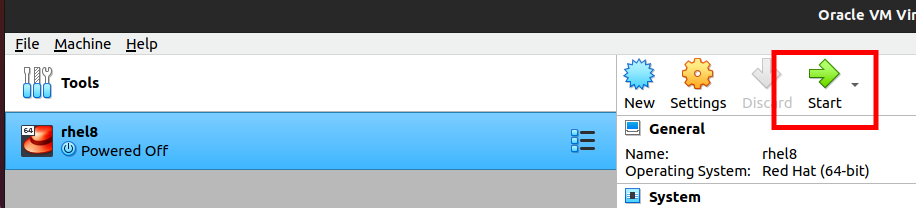
\includegraphics[scale=.3]{content/chapter18/images/image1.2.png}
	\end{figure}		
	
	
 	\item Select the "Install Red Hat Enterprise Linux 8.1.0" option using \textbf{up/down arrow keys on the keyboard}.
 	\begin{figure}[h!]
 		\centering
 		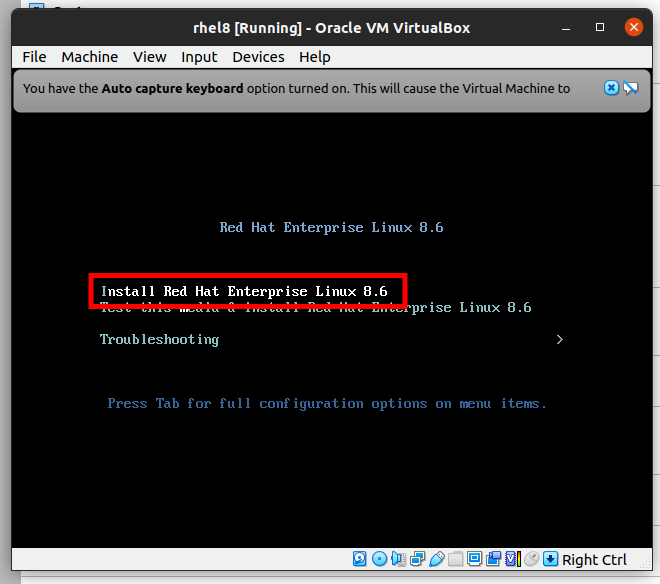
\includegraphics[scale=.2]{content/chapter18/images/image11.png}
 	\end{figure}		


	\item Select the language of your preference and press continue button.
 	\begin{figure}[h!]
		\centering
		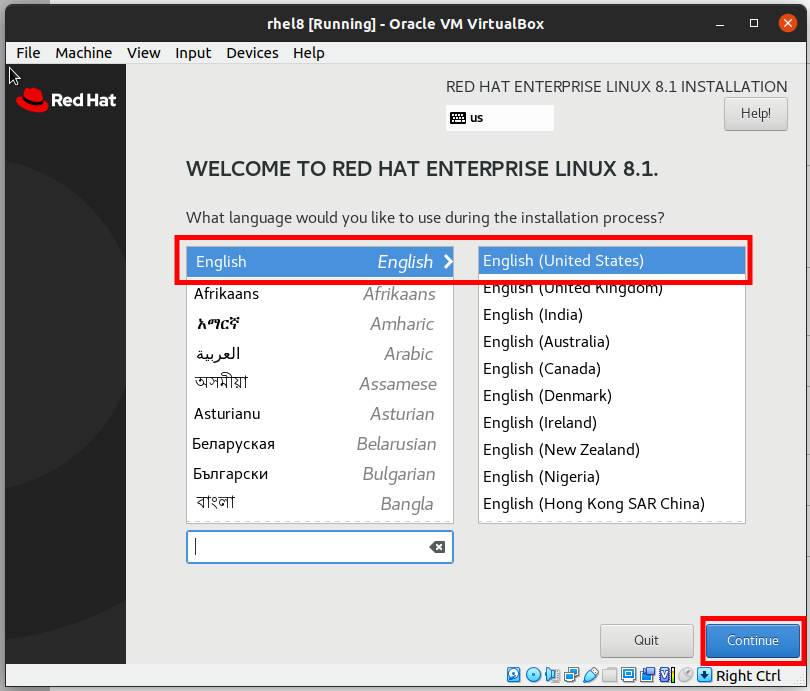
\includegraphics[scale=.2]{content/chapter18/images/image1.1.png}
	\end{figure}		

	\newpage
	
 	\item Select the \textbf{"Installation Destination"} as shown.
	\begin{figure}[h!]
		\centering
		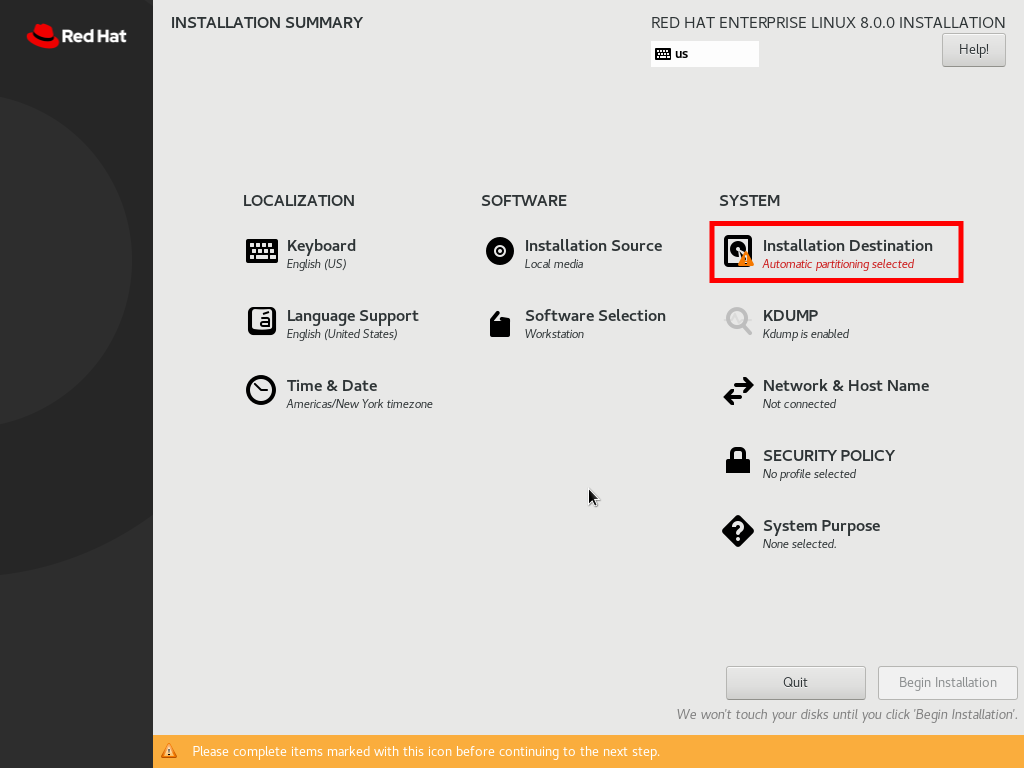
\includegraphics[scale=.2]{content/chapter18/images/image12.png}
	\end{figure}		

 	\item Select the \textbf{"Custom"} option and click on \textbf{"Done"} as shown.
	\begin{figure}[h!]
		\centering
		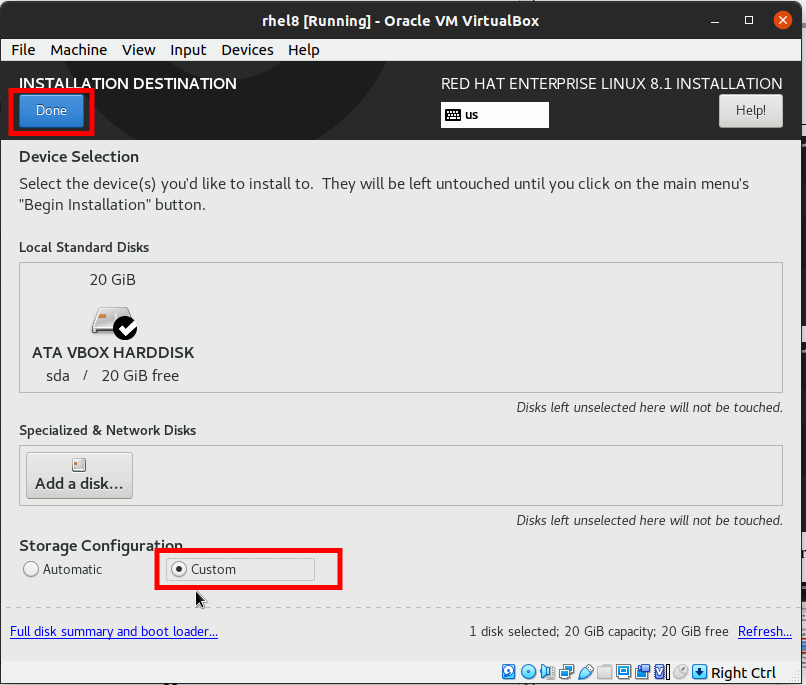
\includegraphics[scale=.25]{content/chapter18/images/image1.3.png}
	\end{figure}
	

 	\item Add new partition by clicking on \textbf{"+"} icon.
	\begin{figure}[h!]
		\centering
		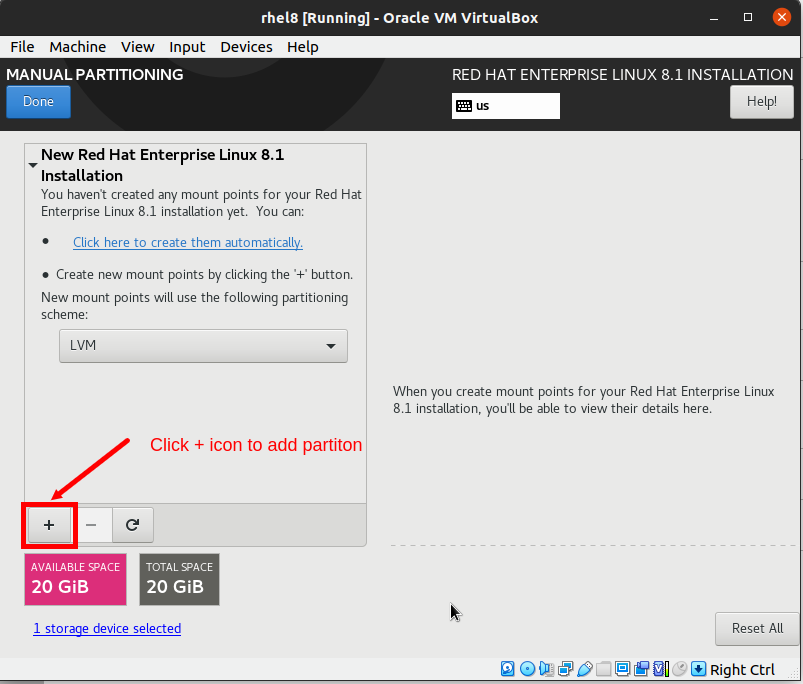
\includegraphics[scale=.2]{content/chapter18/images/image1.5.png}
	\end{figure}
		
 	\item Create \textbf{"/boot"} partition of size \textbf{"512MB"} as shown.
	\begin{figure}[h!]
		\centering
		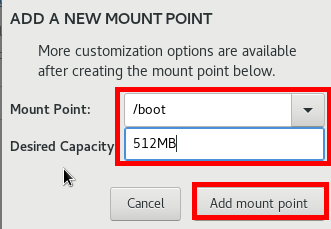
\includegraphics[scale=.4]{content/chapter18/images/image1.6.png}
	\end{figure}		

 	\item Similarly create below partitions:
 	\begin{itemize}
 		\item \textbf{"swap"} partition of size \textbf{"1GB"}
 		\item \textbf{"/var"} partition of size \textbf{"5GB"}
 		\item \textbf{"/home"} partition of size \textbf{"7GB"}
 		\item Remaining space to \textbf{"/"} partition
 	\end{itemize}

	\item You should see summary of all partitions as shown in the image:
	\begin{figure}[h!]
		\centering
		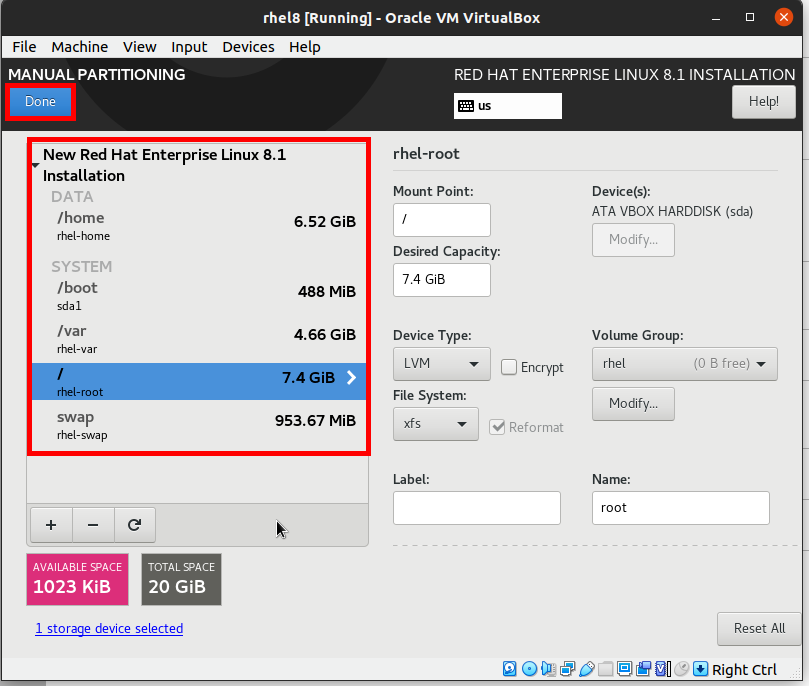
\includegraphics[scale=.2]{content/chapter18/images/summary.png}
		\label{primary_swap1}
	\end{figure}		


 	\item Accept all the changes as shown:
	\begin{figure}[h!]
		\centering
		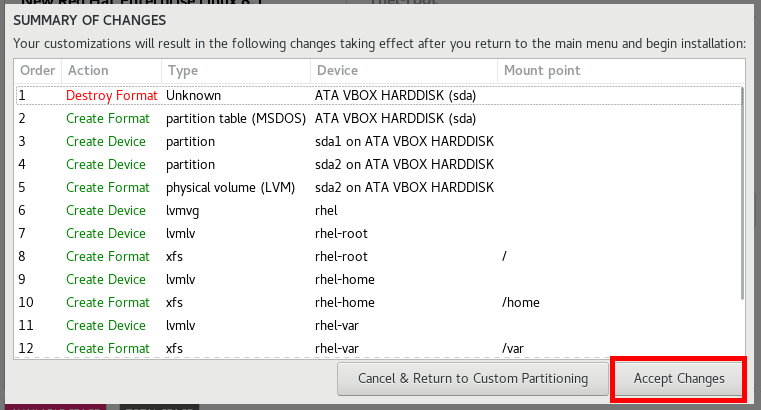
\includegraphics[scale=.3]{content/chapter18/images/accept.png}
	\end{figure}		

	\newpage
	\item Next, select the \textbf{"Software Selection"}:
	\begin{figure}[h!]
		\centering
		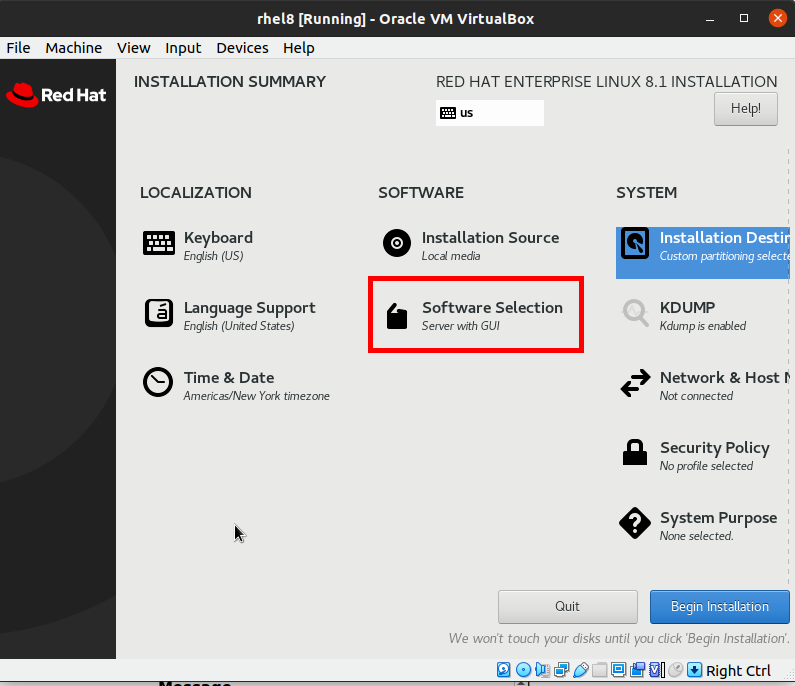
\includegraphics[scale=.3]{content/chapter18/images/server1.png}
	\end{figure}		
	
	\item Select the \textbf{"Server with GUI"} \& \textbf{"Developement Tools"} as highlighted:
	\begin{figure}[h!]
		\centering
		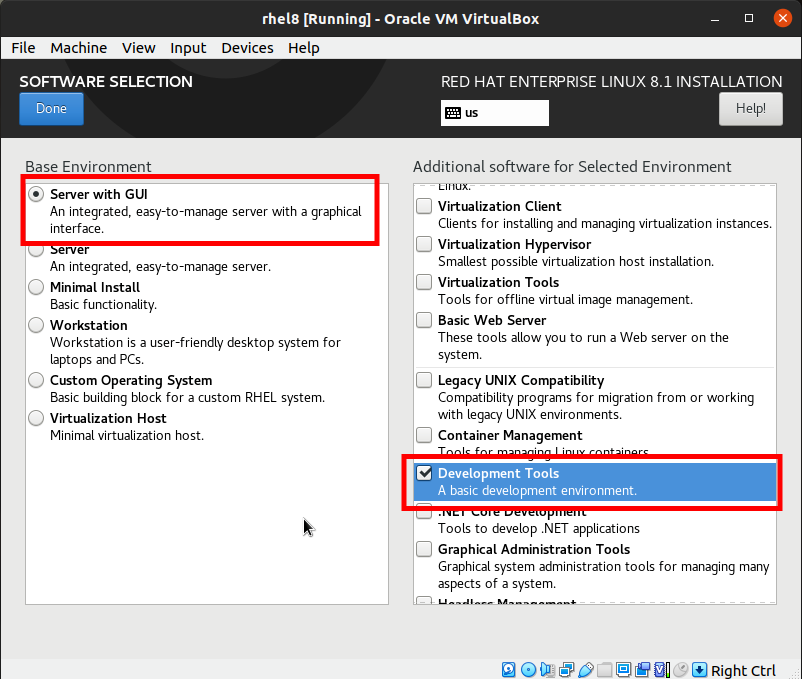
\includegraphics[scale=.3]{content/chapter18/images/server2.png}
		\caption{}
		\label{primary_swap3}
	\end{figure}		
	\newpage
	\item Select the \textbf{"Time and Date"}:
	\begin{figure}[h!]
		\centering
		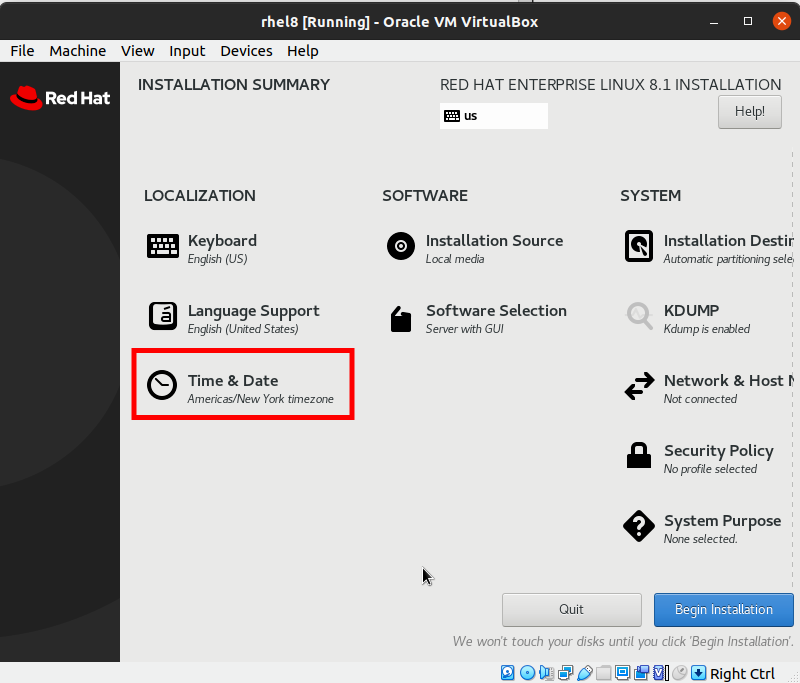
\includegraphics[scale=.3]{content/chapter18/images/server3.png}
	\end{figure}		

	
	
	\item Select appropriate date and time as shown:
	\begin{figure}[h!]
		\centering
		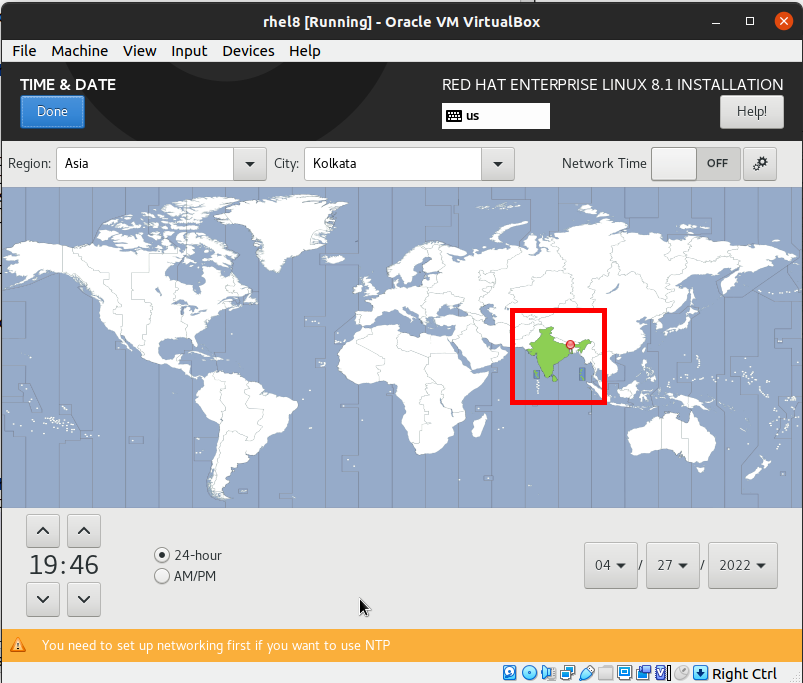
\includegraphics[scale=.3]{content/chapter18/images/server4.png}
	\end{figure}		
	\newpage
	\item Next, select \textbf{"KDUMP"} to disable it:
	\begin{figure}[h!]
		\centering
		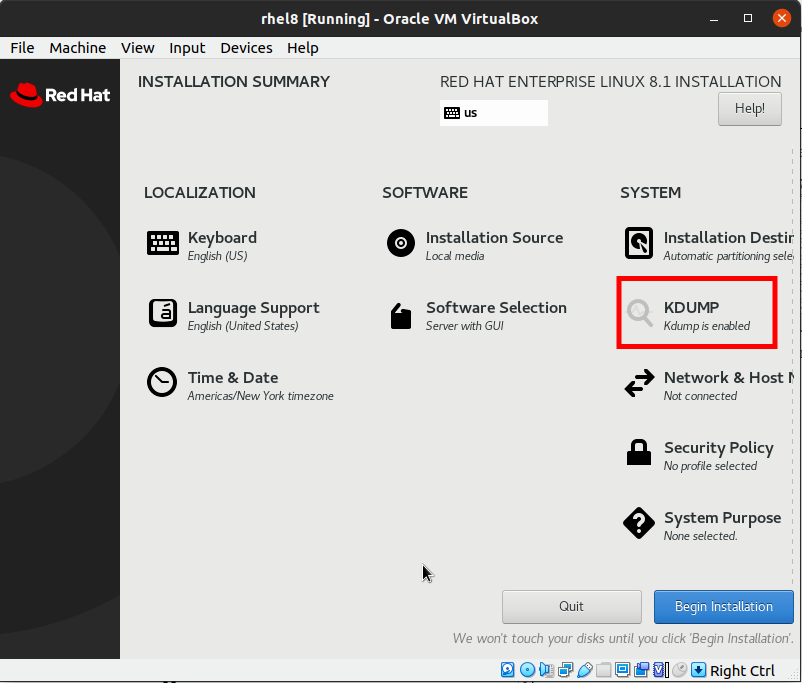
\includegraphics[scale=.25]{content/chapter18/images/server5.png}
	\end{figure}			

	\item Uncheck the \textbf{"Enable kdump"} checkbox to save the memory and click on \textbf{"Done"}:
	\begin{figure}[h!]
		\centering
		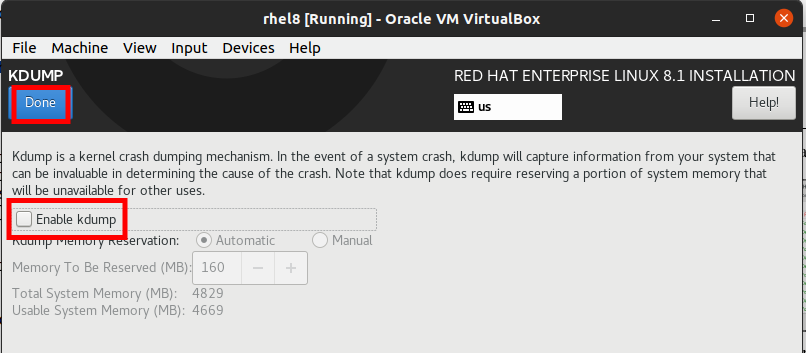
\includegraphics[scale=.3]{content/chapter18/images/kdump.png}
	\end{figure}			

	\item Finally start the installation. During OS installation, set the root password and create user as per your requirement:
	\begin{figure}[h!]
		\centering
		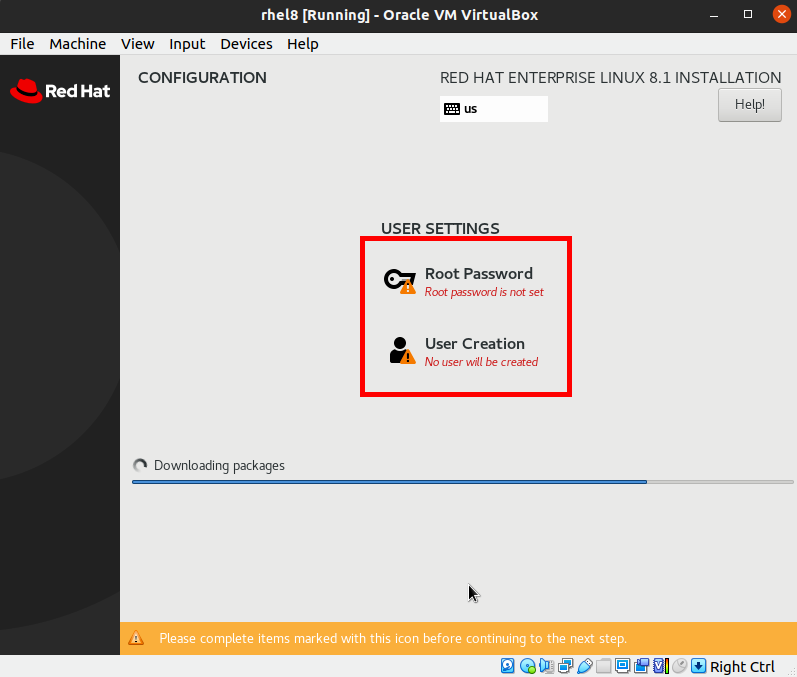
\includegraphics[scale=.25]{content/chapter18/images/server6.png}
	\end{figure}		


 \end{itemize}

\end{flushleft}
